\documentclass[a4paper,12pt]{article}
\usepackage[utf8]{inputenc}
\usepackage[polish]{babel}
\usepackage[OT4]{polski}
 
\usepackage{graphicx}
\graphicspath{ {images/} }
 
\title{Metody odkrywania wiedzy\\\Large{Dokumentacja końcowa}}
\author{Rafał Okuniewski, Maciej Zaborek}
\date{czerwiec 2017}
 
\begin{document}
 
\maketitle
 
\section{Wstęp}
W ramach projektu zajęliśmy się tematem analitycznym dotyczącym regresji na zbiorze danych dokumentującym liczbę wypożyczeń rowerów miejskich.
 
 Celem projektu było zapoznanie się z istniejącymi rozwiązaniami dotyczącymi algorytmów regresji, wykorzystanie ich na dostepnym zbiorze, przeprowadzenie prawidłowych badań tych algorytmów oraz ich dostosowanie w celu osiągnięcia jak najmniejszego błędu na dostępnym zbiorze danych testowych.
 Celem projektu było również wykorzystanie algorytmów umożliwiających ocenę i selekcję atrybutów a także analiza potencjału wprowadzenia nowych atrybutów do zbioru na podstawie analizy istniejących oraz wiedzy pozyskanej ze zbioru.
W ramach przeprowadzonych badań skorzystaliśmy z pięciu dostępnych w języku R algorytmów regresji: regresji liniowej, regresji lokalnej, robust regression z M-estymacją, drzewa regresji oraz regresji z wykorzystaniem algorytmu sieci neuronowej.
 
Przeprowadzona analiza miała na zadaniu znalezienie najlepiej radzącego sobie z postawionym zadaniem algorytmu, jak i zbadaniem wpływu parametrów poszczególnych z nich na otrzymywany wynik.

\section{Zbiór danych}

W projekcie wykorzystano zbiór danych dostępny pod adresem: \\\textit{https://www.kaggle.com/c/bike-sharing-demand/}. Zawiera on dane zebrane na przestrzeni dwóch lat dotyczące ilości wypożyczeń w systemie rowerów miejskich. Każda próbka to opis każdej godziny pracy systemu w ciągu dnia. Atrybuty zbioru to kolejno:
\begin{itemize}
	\item data \textit{datetime}
	\item pora roku \textit{season}
	\item czy dany dzień jest świętem \textit{holiday}
	\item czy dany dzień jest dniem roboczym \textit{workingday}
	\item pogoda - jedna z czterech wartości \textit{weather}
	\item temperatura \textit{temp}
	\item temperatura odczuwalna \textit{atemp}
	\item wilgotność \textit{humidity}
	\item prędkość wiatru \textit{windspeed}
	\item liczba rozpoczetych wypożyczeń niezarejestrowanych użytkowników \textit{casual}
	\item liczba rozpoczętych wypożyczeń przez zarejestrowanych użytkowników \textit{registered}
	\item całkowita liczba wypożyczeń - atrybut ciągły podlegający pomiarowi błędu \textit{count}
\end{itemize}

W każdym miesiącu pierwszych 19 dni stanowią dane uczące zbioru. Celem przeprowadzanej regresji jest przewidzenie liczby wypożyczonych rowerów w każdej godzinie od dnia 20. każdego miesiąca, który stanowi zbiór danych testowych.

\section{Wstępne przetwarzanie danych}
Wykorzystane dane pochodzą z platformy Kaggle i są w formie, która nie wymagała uzupełnienia, ponieważ są one kompletne.
 
W trakcie wstępnego przetwarzania danych dodawane są nowe atrybuty (plik Preprocess.R):
    \begin{itemize}
        \item
            Dzień tygodnia (funkcja addDayAttr(), atrybut "weekdays")
        \item
            Godzina (funkcja addHourAttr(), atrybut "hours")
        \item
            Czy w drodze do/z pracy (godzina 7-9 oraz 15-18 w dniu roboczym) (funkcja addWorkWayAttribute(), atrybut "onwaytowork")
    \end{itemize}

Motywacją dla wprowadzenia nowych atrybutów był fakt, iż charakter liczby wypożyczeń w dni robocze oraz w weekend jest odmienny i silnie zależny od godziny dnia.

\begin{figure}[!htb]
    \center
    \scalebox{0.8}{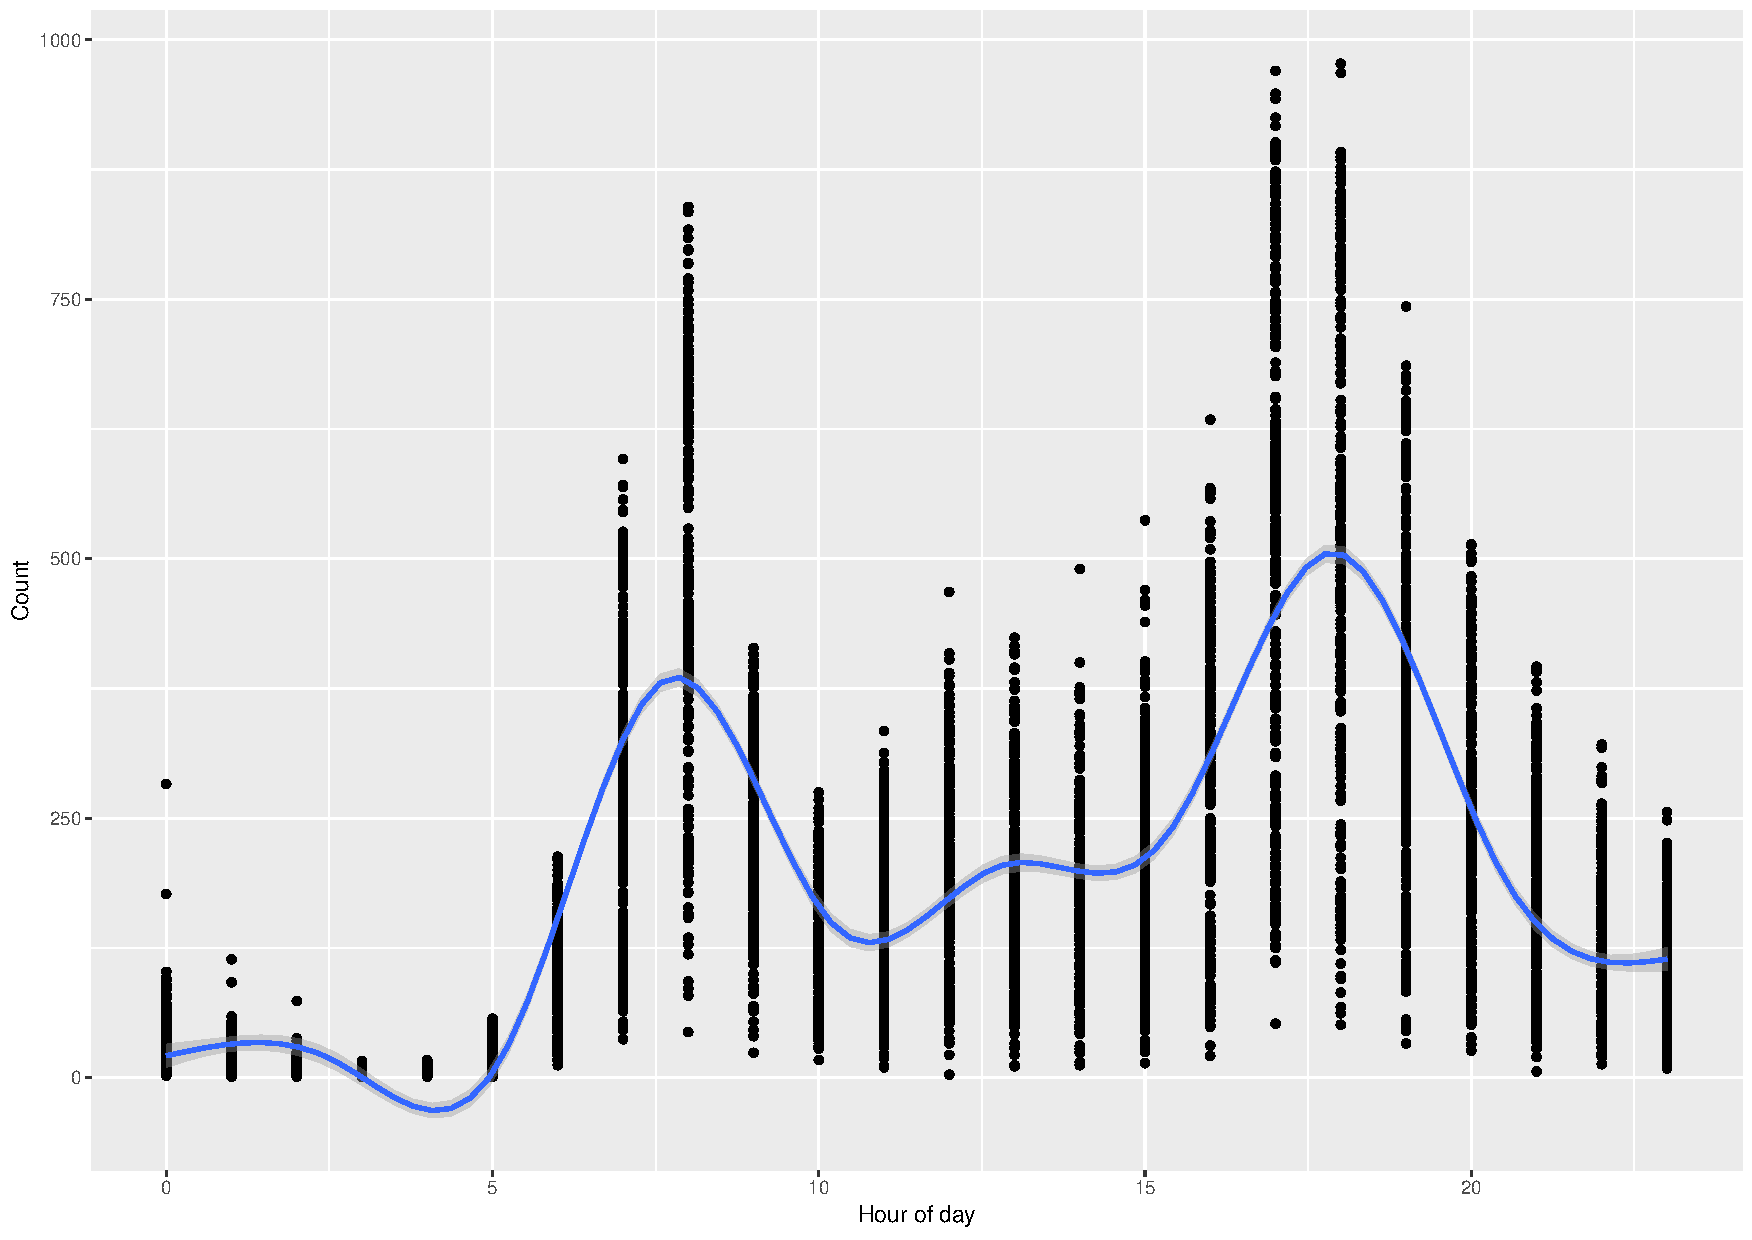
\includegraphics[width=0.8\textwidth]{CountVsHourWorkDays}}
    \caption{Wypożyczenia w dni robocze}
\end{figure}

\begin{figure}[!htb]
    \center
    \scalebox{0.8}{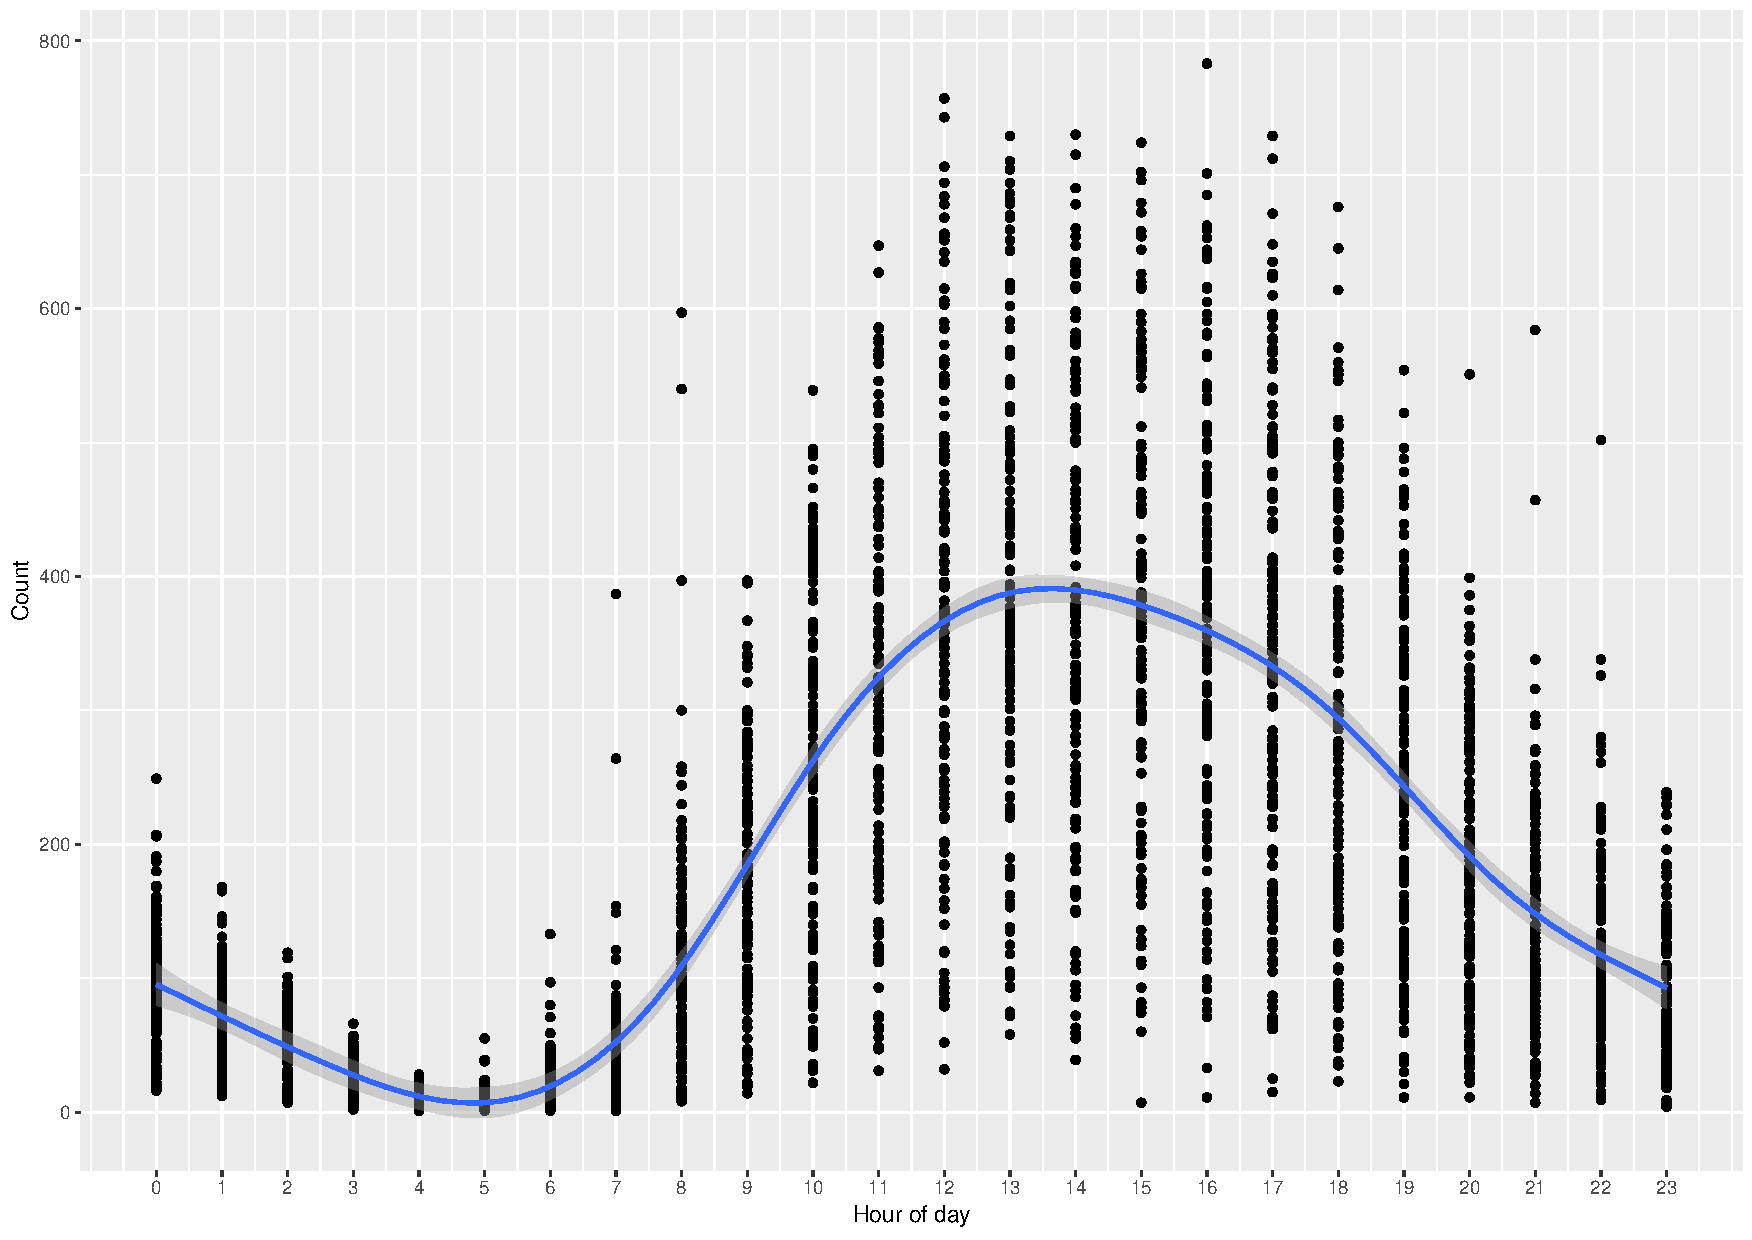
\includegraphics[width=0.8\textwidth]{CountVsHourNotWorking}}
    \caption{Wypożyczenia poza dniami roboczymi}
\end{figure}
    
Usuwane są również ze zbioru trenującego atrybuty dotyczące liczby wypożyczonych rowerów przez zarejestrowanych i niezarejestrowanych użytkowników, ponieważ dane te nie są dostępne w zbiorze testowym.

Dla wykorzystywanego do uczenia zbioru zastosowano wstępną obróbkę, która ograniczała się do usunięcia odstających danych. Ze zbioru uczącego usuwane były przykłady, dla których kwadrat odległości od średniej przekraczał trzykrotność odchylenia standardowego. Zbiór w ten sposób uległ redukcji o około 1\%.

\section{Algorytmy selekcji atrybutów}

    Przed przystąpieniem do selekcji atrybutów przeprowadzona została analiza macierzy kowariancji wszystkich atrybutów. Wykazała ona
    spodziewaną, wysoką zależność pomiędzy atrybutami związanymi z pogodą, w szczególności atrybutami "temp" i "atemp" (temperatura faktyczna i odczuwalna),
    co sugeruje wykorzystanie do celów regresji wyłącznie jednego z nich.
    
    \subsection{Stepwise Regression}
    
        Do selekcji atrybutów wykorzystano regresję krokową. Użyto metody \texttt{stepAIC} z pakietu \texttt{MASS}. Wykorzystano dwukierunkowy wariant algorytmu (\textit{direction = "both"}).
        Dla początkowego modelu zawierającego wszystkie atrybuty w postaci:
        
        $count ~ onwaytowork + hours + weekdays + windspeed + humidity + atemp + temp + weather + workingday + holiday + season$
        
        otrzymano model końcowy w postaci:
        
        $count ~ onwaytowork + hours + weekdays + windspeed + humidity + atemp + workingday + season$
        
        W kolejnych krokach usuwane są następująco atrybuty: \textit{holiday}, \textit{weather} praz \textit{temp}.
       
    \subsection{Regsubset analisys}
        Algorytm selekcji atrybutów korzystający z wyszukiwania wyczerpującego. Wykorzystano funkcję \texttt{stepAIC} z pakietu \texttt{leaps}. Wynikiem jej działania są najlepsze modele dla odpowiedniej liczby atrybutów. Wyniki działania przedstawione są na rysunku \ref{fig:regsubset}. Wynika z niego, że model z sześcioma atrybutami jest najkorzystniejszy. Modele z większą liczbą atrybutów zostały ocenione nieznacznie lepiej.
        \begin{figure}[h]
            \centering
            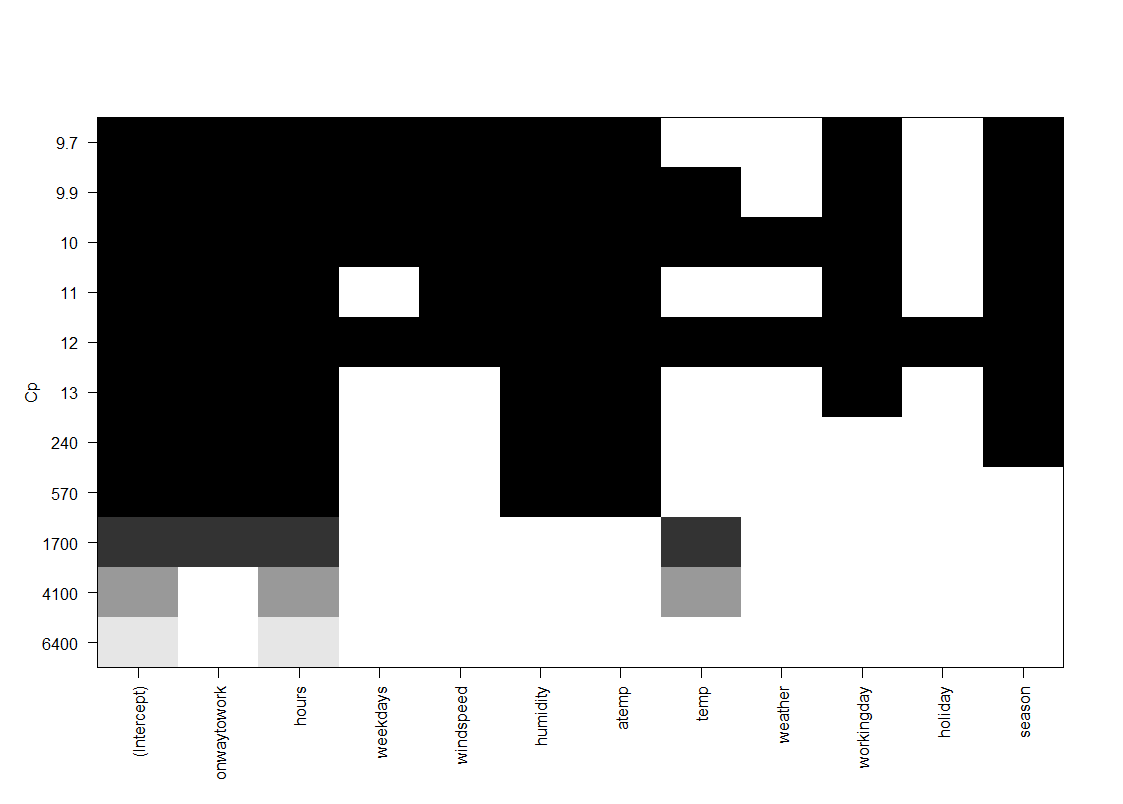
\includegraphics[width=\linewidth]{regsubsetanalysis}
            \caption{Wyniki regsubset analisys}
            \label{fig:regsubset}
        \end{figure}
        
     \subsection{Algorytm RFE}
     Algorytm RFE (\textit{Recursive Feature Elimination}) wykorzystuje zewnętrzny algorytm (w tym przypadku regresję liniową) do oceny błędu walidacji skrośnej. po wykonaniu walidacji bada wagi przypisane poszczególnym atrybutom a następnie przycina atrybuty o najniższych wagach.  W każdym kroku algorytmu wykorzystywany jest coraz mniejszy podzbiór atrybutów aż do momentu, gdy zostanie osiągana żądana liczba atrybutów.
     Wykorzystanie algorytmu \texttt{rfe} z pakietu \texttt{caret} umożliwiło przeprowadzenie rankingu istniejących w zbiorze atrybutów:
     \begin{enumerate}
         \item hours
         \item humidity
         \item onwaytowork
         \item weather
         \item weekdays
         \item season
         \item workingday
         \item temp
         \item atemp
      \end{enumerate}
      Algorytm pozwala również przyjrzeć się zależności błędu od liczby wykorzystywanych atrybutów:

     \begin{figure}[!htb]
        \center
        \scalebox{0.8}{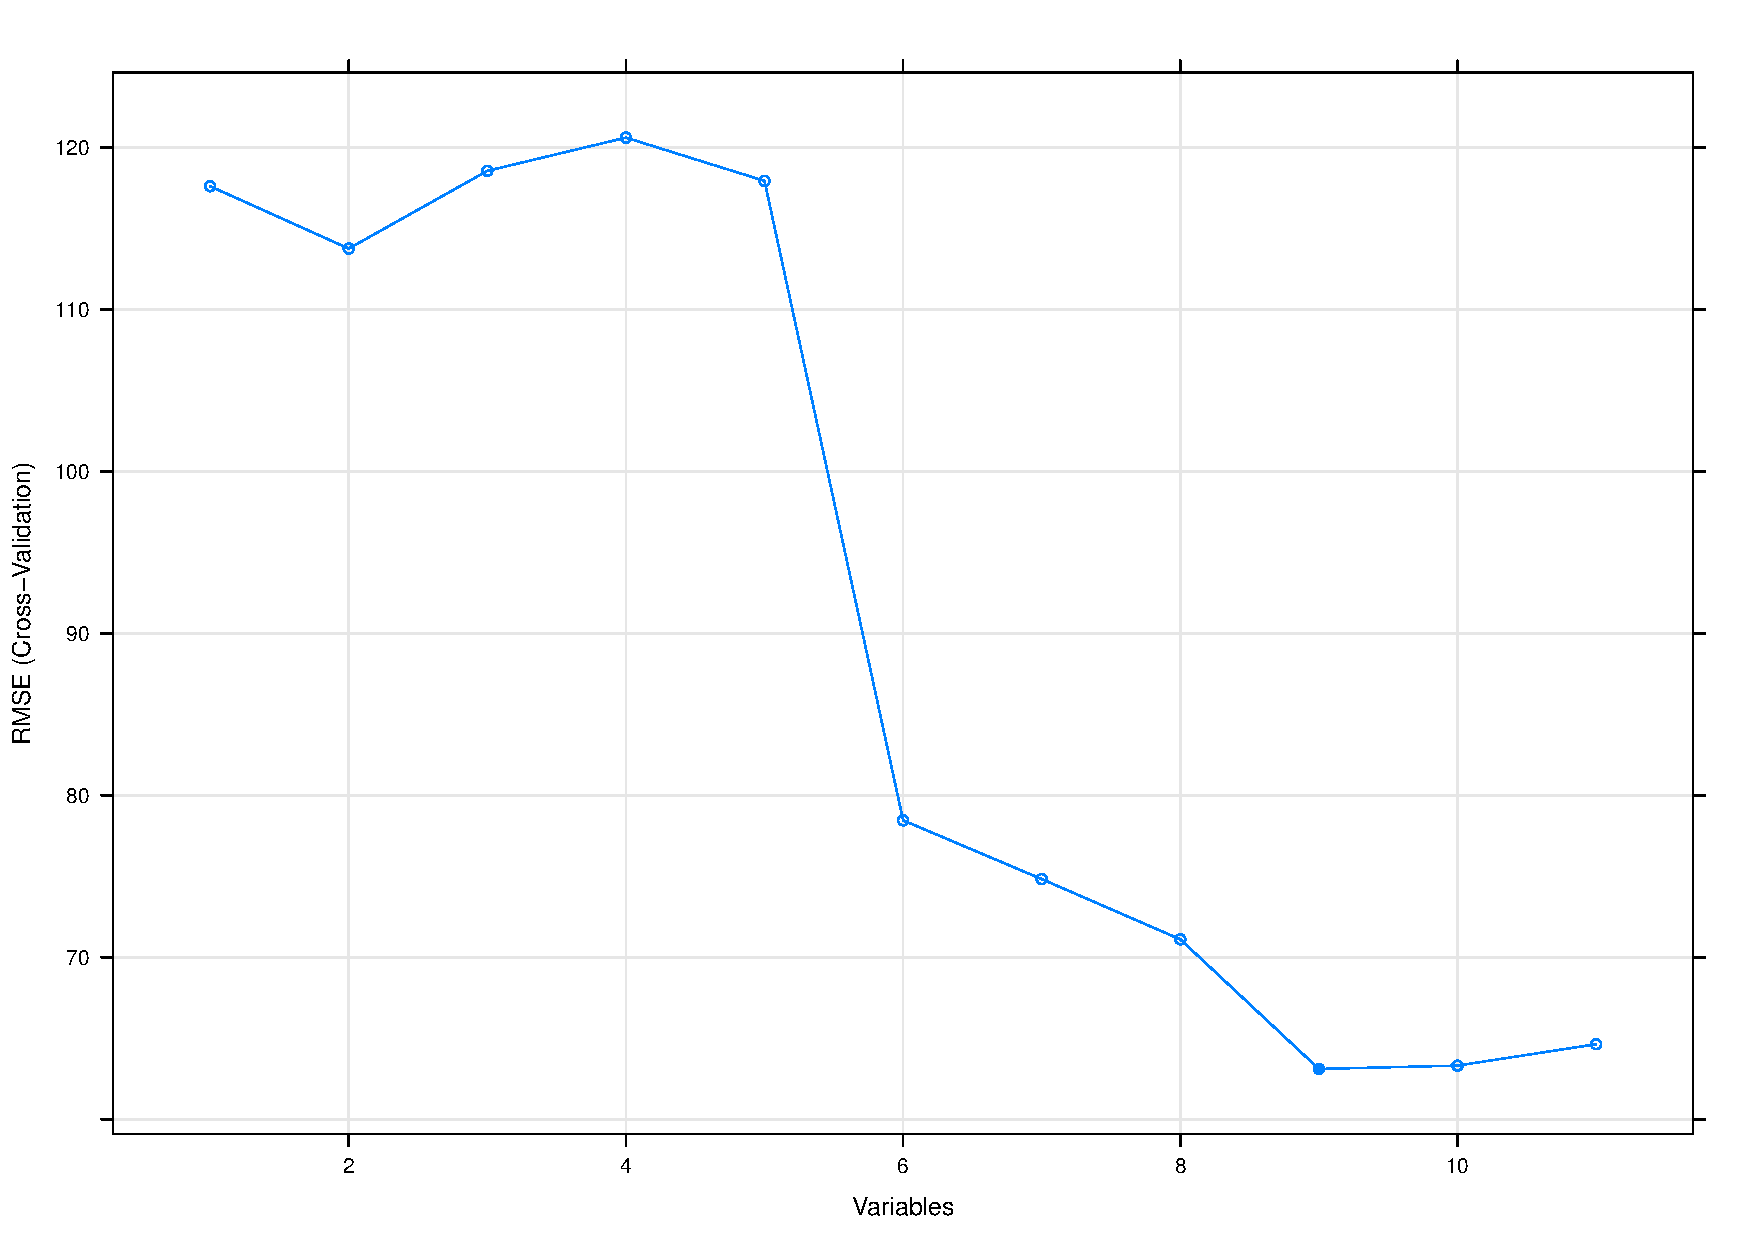
\includegraphics[width=0.8\textwidth]{RFEAnalysis}}
        \caption{Błąd w zależności od liczby atrybutów}
    \end{figure}
       Wyniki działania algorytmu pokazują, że optymalną liczbą wykorzystywanych atrybutów jest 6-8, przy większej ich liczbie spadek błędu wskutek
       dodania nowego atrybutu jest marginalny.
\section{Metody oceny algorytmów}

    \subsection{Miary błędów}
    Dla każdego rodzaju walidacji z wyjątkiem walidacji na zbiorze testowym (przeprowadzanej za pomocą aplikacji Kaggle) obliczano dwie miary błędu:
    \begin{enumerate}
        \item Pierwiastek z błędu średniokwadratowego logarytmicznego $$RMSLE = \sqrt{\frac{1}{n}\sum_{n}^{i=1}(log(p_i + 1) - log(a_i + 1))^2}$$

        \item Pierwiastek z błędu średniokwadratowego $$RMSE = \sqrt{\frac{1}{n}\sum_{i=1}^{n}(y_i - \hat{y_i})^2}$$
     \end{enumerate}
    Aplikacja Kaggle oceniała wyłącznie błąd $RMSLE$ na zbiorze testowym.
    
    \subsection{Walidacja skrośna}
    Algorytmy badano wykorzystując algorytm k-krotnej walidacji skrośnej. Polega ona na podziale zbioru na K podzbiorów, a następnie wykonywaniu na nich 
    walidacji, przy czym w każdym kroku jeden z K zbiorów pełni rolę zbioru testowego, zaś pozostałe pełnią role zbioru uczącego. W przypadku $ K = N$, a zatem gdy zbiór uczący jest równy w każdym kroku całemu dostępnemu zbiorowi treningowemu z wyjątkiem jednej obserwacji, walidacja skrośna k-krotna staje się walidacją \textit{leave-one-out}. Umożliwia ona lepsze uniezależnienie wyników eksperymentu od zmiennych losowych. Dostępny zbiór treningowy okazał się jednak na tyle duży, iż zespół nie wykrył istotnych różnic w błędzie otrzymywanym podczas walidacji metodą leave-one-out oraz zwykłej walidacji skrośnej. Dla każdego algorytmu 
    badano średni błąd przy walidacji dla k=5.
    \subsection{Walidacja na zbiorze testowym}       
    Na stronie Kaggle wraz z treścią zadania i zbiorem trenującym udostępniony również został zbiór testowy, pozbawiony liczby wypożyczeń. 
    Zbiór ten zawierał łącznie 6494 wpisy, które stanowią zapis liczby wypożyczeń co godzinę w dniach 20-31 każdego miesiąca w okresie dwóch lat
    (w odróżnieniu od zbioru trenującego, który zawierał wpisy z dni 1-19 każdego miesiąca).
    Po wytrenowaniu
    modeli na całym zbiorze trenującym dokonywano predykcji na zbiorze testowym, a następnie ładowano go do aplikacji Kaggle. Odnotowywany został błąd 
    $RMSLE$ zwrócony przez aplikację. Badano w ten sposób zarówno średnią z predykcji wszystkich algorytmów, jak i predykcję poszczególnych algorytmów.
    
    
\section{Przetestowane algorytmy regresji}

   \subsection{Regresja liniowa}
       Dla zbadania regresji liniowej wykorzystano funkcję \texttt{lm} z pakietu {stats}.
       Przy wykorzystaniu pełnego zbioru atrybutów model liniowy dał następujące błędy w walidacji skośnej dla k = 5:
       RMSLE 1.151384
       RMLE 119.815
        Wykorzystane w modelu współczynniki dla poszczególnych atrybutów widoczne są w tabeli \ref{tab:wspolczynnikiLin}.
        
            \begin{table}
            	\centering
            	\begin{tabular}{|c|c|c|c|}
            	\hline 
            	(Intercept) & onwaytowork & hours & weekdays \\ 
            	\hline 
            	34.7226629 & 233.2879647 & 8.3635308 & 1.2258257 \\ 
            	\hline 
            	windspeed & humidity & atemp & temp \\ 
            	\hline 
            	0.3128109 & -2.3272347 & 5.0743702 & 1.2704038 \\ 
            	\hline 
            	weather & workingday & holiday & season \\ 
            	\hline 
            	-2.7714344 & -34.6009805 & -1.8851859 & 20.1173451 \\ 
            	\hline 
            	\end{tabular} 
                \caption{Współczynniki w modelu liniowym}
                \label{tab:wspolczynnikiLin}
        \end{table}  
        
        Dla modelu zwróconego przez algorytm \textit{stepwise regression} błąd wynosił odpowiednio:
        RMSLE 1.151384
        RMLE 119.815
        
        Tabela \ref{tab:linModels} zawiera błędy dla wybranych modeli zwróconych przez algorytm \textit{Regsubset analisys}. Wyniki pokrywają się z klasyfikacją modeli podaną jako wynik jego działania. Dla modeli składających się z 6 i więcej atrybutów błąd maleje minimalnie. Dla modelu składającego się z 8 atrybutów otrzymujemy już taki sam błąd jak dla pełnego zestawu atrybutów.
        
        \begin{table}[h]
        	\centering
            \begin{tabular}{|p{2cm}|p{8cm}|r|r|}
                \hline
                Liczba atrybutów & atrybuty & RMSLE & RMSE \\
                \hline
                1 & 
                hours
                & 
                1.328705
                & 
                152.3693
                \\
                \hline
                2 & 
                hours + temp
                & 
                1.236916
                & 
                141.8473
                \\
                \hline
                3 & 
                onwaytowork + hours + temp
                & 
                1.18398
                & 
                129.6105
                \\
                \hline
                4 & 
                onwaytowork + hours + humidity + atemp
                & 
                1.172317
                & 
                123.351
                \\
                \hline
                5 &  onwaytowork + hours + humidity + atemp + season
                & 
                1.171745
                & 
                121.2109
                \\
                \hline
                7 & onwaytowork + hours + windspeed + humidity + atemp + workingday + season & 
                1.152467
                & 
                119.855
                \\
                \hline
                8 & 
                onwaytowork + hours + weekdays + windspeed + humidity + atemp + workingday + season 
                & 
                1.15163
                & 
                119.8403
                \\
                \hline
            \end{tabular}
            \caption{Błąd funkcji lm dla poszczególnych podzbiorów atrybutów zwróconych przez regsubset}
            \label{tab:linModels}
        \end{table}
        
        
    \subsection{Regresja lokalna}
        Jako metodę regresji lokalnej wykorzystano funkcję \texttt{loess} z pakietu \texttt{stats}. Przyjmuje ona do czterech atrybutów. Funkcja przyjmuje dwa parametry, które dotyczą wygładzania:
        \begin{itemize}
            \item
                Degree - stopień wielomianów stosowanych w wygładzaniu wielomianów. Przyjmuje watości 0, 1 oraz 2.
            \item
                Span - parametr $\alpha$ odpowiadający za stopień wygładzania
        \end{itemize}
        
        W tabeli \ref{tab:loess} przedstawiono wyniki badań jakości przeprowadzonej regresji lokalnej. Błędy zostały policzone jako średnia błędów z walidacji skośnej dla k = 5. Choć mniejszy błąd występował dla wielomianów drugiego stopnia, to najlepszy wynik osiągnięto dla \textit{Degree} = 1 oraz \textit{span} = 0.01. Im mniejsza była wartość parametu \textit{span}, tym mniejszy był błąd walidacji skośnej.
        
        
        \begin{table}[h]
        	\centering
            \begin{tabular}{|c|c|c|c|}
                \hline
                Degree & Span & RMSLE & RMSE \\
                \hline
                2 & 0.01 & 0.78
                & 99.7 \\
                \hline
                1 & 0.01 & 0.75 & 99.2 \\
                \hline
                0 & 0.01 & 0.83 & 104 \\
                \hline
                2 & 0.1 & 0.932 & 112 \\
                \hline
                1 & 0.1 & 1 & 114 \\
                \hline
                0 & 0.1 & 1.12 & 121 \\
                \hline
                2 & 0.3 & 1.02 & 114 \\
                \hline
                1 & 0.3 & 1.22 & 121 \\
                \hline
                0 & 0.3 & 1.25 & 131 \\
                \hline
                2 & 0.5 & 1.12 & 117 \\
                \hline
                1 & 0.5 & 1.23 & 124 \\
                \hline
                0 & 0.5 & 1.32 & 136 \\
                \hline
                2 & 0.75 & 1.27 & 119 \\
                \hline
                1 & 0.75 & 1.17 & 128 \\
                \hline
                0 & 0.75 & 1.38 & 142 \\
                \hline
                2 & 1 & 1.4 & 120 \\
                \hline
                1 & 1 & 1.14 & 133 \\
                \hline
                0 & 1 & 1.5 & 157 \\
                \hline
            \end{tabular}
            \caption{Błąd funkcji loess w zależności od przyjętych parametrów dla formuły count \~ humidity + hours + atemp}
            \label{tab:loess}
        \end{table}
        
        Wpływ doboru atrybutów na wyniki regresji lokalnej przedstawia tabela \ref{tab:loessAttr}. Najlepszy wynik osiągnięto dla dwóch atrybutów: \textit{hours} i \textit{temp}.
        
        \begin{table}
        	\centering
            \begin{tabular}{|c|c|c|}
                \hline 
                atrybuty & RMSLE & RMSE \\ 
                \hline 
                hours & 4.774647 & 247.5403 \\ 
                \hline 
                hours + temp & 0.7036961 & 100.3796 \\ 
                \hline 
                hours + humidity + atemp + season & 0.8488961 & 199.1475 \\ 
                \hline 
            \end{tabular}
            \caption{Wyniki funkcji \texttt{loess} w zależności od dobranych atrybutów dla parametrów \textit{span} = 0.01 \textit{degree} = 1}
            \label{tab:loessAttr}
        \end{table}
        
   \subsection{Robust regression z M-estymacją}
   
   Regresja typu ''robust'' z M- lub MM-estymacją wykazuje zwiększoną odporność na zanieczyszczone dane trenujące, zawierające dużą liczbę wartości odstających. W przypadku 
   dostępnego zbioru treningowego nie było to dużym problemem, ponieważ w procesie preprocessingu usunięte zostały takie wartości, zaś ich ogólna liczba była niewielka.
   
    \begin{table}
    \centering  
   \begin{tabular}{|c|c|c|}
   \hline
   Sposób estymacji & RMSLE & RMSE \\
   \hline
   M-estymacja & 1.129622 & 120.9462 \\
   \hline
   MM-estymacja & 1.110996 & 122.7891 \\
   \hline
   \end{tabular}
   \caption{Wyniki w zależności od metody estymacji (średni błąd walidacji skrośnej dla k=5)}
    \end{table}
    \begin{table}
    	\centering
            \begin{tabular}{|c|c|c|}
                \hline
                Funkcja psi & RMSLE & RMSE \\
                \hline
                psi.bisquare & 1.116625 & 122.184 \\
                \hline
                psi.huber & 1.129622 & 120.9462 \\
                \hline
                psi.hampel & 1.14003 & 120.229 \\
                \hline
            \end{tabular}
            \caption{Wyniki w zależności od funkcji psi}    
    \end{table}
    
    \begin{figure}[!htb]
        \center
        \scalebox{0.8}{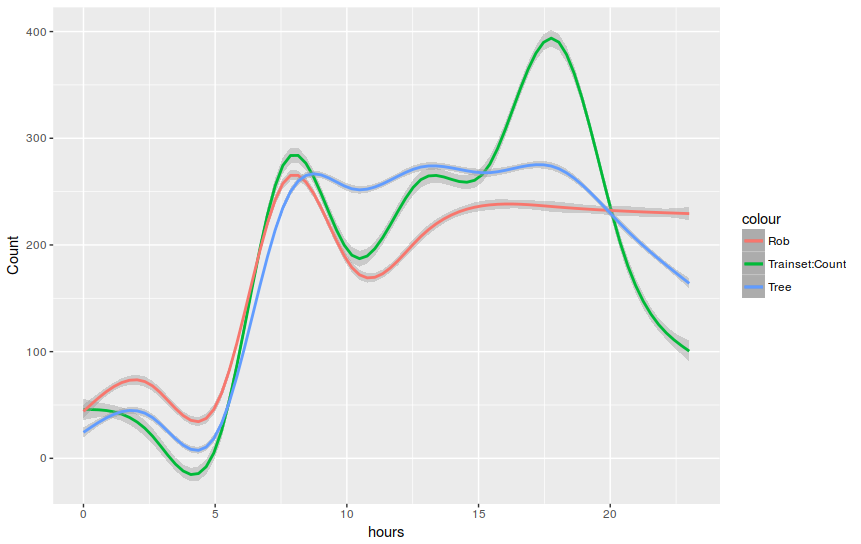
\includegraphics[width=0.8\textwidth]{robust1}}
        \caption{Wyniki regresji w trakcie weekendu w porównaniu z innymi algorytmami}
    \end{figure}
    
    Regresja z m-estymacją powoduje wygładzenie skokowych zmian wartości liczby wypożyczeń, co  szczególnie negatywnie odbija się dla danych pochodzących z dni roboczych (szczyt poranny i popołudniowy). Wobec tego, przeprowadzono porównanie błędu obliczonego z wykorzystaniem tej metody dla danych weekendowych oraz dla danych z dni roboczych oraz porównano je z inną metodą wyznaczania regresji

    \begin{table}
    	\centering
        \begin{tabular}{|c|c|c|}
                \hline
                & Dni robocze & Weekendy \\
                \hline
                Robust RMSE & 120.8319 & 123.9919 \\
                \hline
                Robust RMSLE & 1.034289 & 1.258234 \\
                \hline
                Linear RMSLE & 1.097582 & 1.265375 \\
                \hline
        \end{tabular}
        \caption{Porównanie wyników osiąganych przez algorytm w dni robocze oraz weekendy}
    \end{table}
    
    Podejście okazało się jednak błędne, ponieważ dla weekendów istniało zbyt mało danych, aby skoki wypożyczeń w godzinach popołudniowych nie uległy wygładzeniu przez algorytm.
    
    \begin{figure}[!htb]
        \center
        \scalebox{0.8}{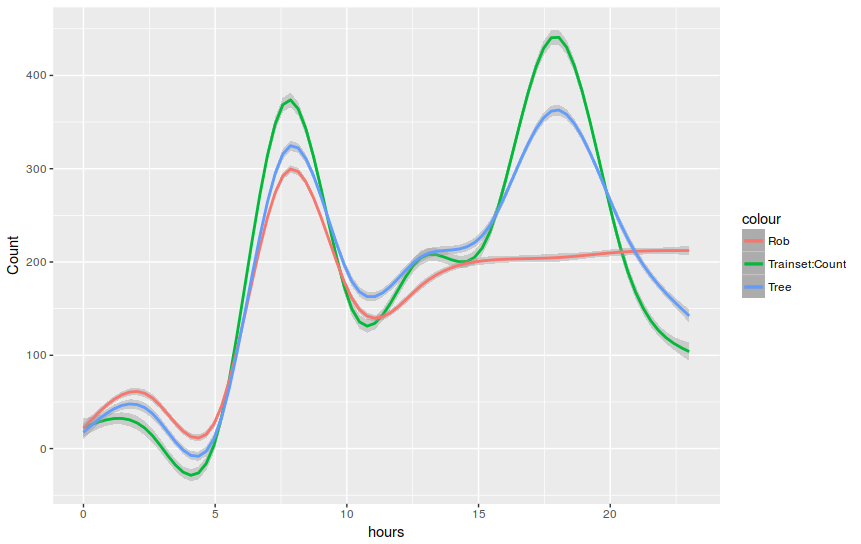
\includegraphics[width=0.8\textwidth]{robust2}}
        \caption{Wykres ukazujący wyniki algorytmu na zbiorze ograniczonym do dni roboczych w porównaniu z innymi algorytmami}
    \end{figure}
    
Po analizie wyjścia algorytmów selekcji atrybutów przeprowadzone zostało badanie algorytmu dla zbioru ograniczonego do 8 atrybutów - "hours"    "humidity"  "onwaytowork" "weather" "weekdays"  "season" "workingday"  "temp", po czym zbiór ten zmniejszano w kolejności od najmniej istotnego atrybutu wg. Algorytmu RFE
    
    \begin{table}
    	\centering
        \begin{tabular}{|c|c|c|}
                \hline
                Liczba atrybutów & RMSLE & RMSE \\
                \hline
                8 & 1.114278 & 122.9576 \\
                \hline
                7 & 1.125025 & 140.3991 \\
                \hline
                6 & 1.132462 & 137.4054 \\
                \hline
                5 & 1.127936 & 138.382 \\
                \hline
                4 & 1.137699 & 138.9563 \\
                \hline
                3 & 1.129964 & 142.1899 \\
                \hline
                2 & 1.190753 & 150.9452 \\
                \hline
                1 & 1.22215 & 155.4499 \\
                \hline
        \end{tabular}
        \caption{Błędy robust regression w zależności od liczby atrybutów.}
    \end{table}
    
    W przypadku regresji robust ograniczenie ilości atrybutów prowadzi do spadku jakości regresji ze względu na niemożliwość dopasowania hiperpłaszczyzny regresji.
    
   \subsection{Drzewa regresji}
       Jako drzewo decyzyjne wykorzystano implementację z pakietu \texttt{rpart}. Na otrzymanym drzewie przeprowadzono przycinanie metodą \texttt{prune}.
       W tabeli \ref{tab:regtree1} przedstawiono wpływ współczynnika przycinania na otrzymane wyniki. Eksperyment przeprowadzono dla wykorzystania w drzewie analizy wariancji (\textit{anova}) oraz rozkładu Poissona (\textit{poissson}). Korzystniejsze wyniki były otrzymywane przy wykorzystaniu rozkładu Poissona.
        \begin{table}
        	\centering
            \begin{tabular}{|c|c|c|c|}
                \hline
                Cp & Meth & RMSLE & RMSE \\
                \hline
                0.005 & anova & 0.8742775 & 98.55746 \\
                \hline
                0.01 & anova & 0.8742775 & 98.55746 \\
                \hline
                0.01 & poisson & 0.7644792 & 100.8667 \\
                \hline
                0.04 & anova & 0.9474914 & 124.1835 \\
                \hline
                0.04 & poisson & 0.941012 & 123.5936 \\
                \hline
                1 & anova & 0.9910873 & 135.782 \\
                \hline
            \end{tabular}
            \caption{Błędy drzewa decyzyjnego}
            \label{tab:regtree1}
        \end{table}
        
        W tabeli \ref{tab:regtree2} przedstawiono wpływ liczby atrybutów na wynik regresji.
        
        \begin{table}
        	\centering
            \begin{tabular}{|c|c|c|}
                \hline
                Liczba atrybutów & RMSLE & RMSE \\
                \hline
                8 & 0.9396421 & 121.915 \\
                \hline
                7 & 0.9301871 & 120.8053 \\
                \hline
                6 & 0.9301871 & 120.8053 \\
                \hline
                5 & 0.9596607 & 128.2725 \\
                \hline
                4 & 0.9596607 & 128.2725 \\
                \hline
                3 & 0.9596607 & 128.2725 \\
                \hline
                2 & 0.9596607 & 128.2725 \\
                \hline
                1 & 0.9596607 & 128.2725 \\
                \hline
            \end{tabular}
            \caption{Błędy drzewa regresji w zależności od liczby atrybutów dla poarametru przycinania \textit{cp} = 0.04 oraz przy wykorzystaniu analizy wariancji.}
            \label{tab:regtree2}
        \end{table}
    
    \subsection{Sieć neuronowa}

    Jako kolejną z metod regresji wykorzystano sieć neuronową. Aby mogła ona zostać wykorzystana w tym celu, neuron w warstwie wyjściowej musi wykorzystywać
    liniową funkcję aktywacji. W celu przeprowadzenia regresji wykorzystano pakiet \texttt{nnet}, który umożliwia zbudowanie sieci neuronowej z pojedynczą
    warstwą ukrytą. W przypadku sieci neuronowej kluczowy był również wynik badania z wykorzystaniem zbioru testowego, ponieważ w przypadku walidacji
    skrośnej zachodziło niebezpieczeństwo zbytniego dopasowania do zbioru trenującego.
        \begin{table}
        	\centering
            \begin{tabular}{|c|c|c|}
            \hline 
            Liczba neuronów & RMSLE & RMSE \\ 
            \hline 
            10 & 0.7643461 & 76.37187 \\ 
            \hline 
            20 & 0.6713900 & 76.48027 \\ 
            \hline 
            30 & 0.5563560 & 63.62175 \\ 
            \hline 
            50 & 0.5327608 & 61.13144 \\ 
            \hline 
            100 & 0.4799462 & 57.26756 \\ 
            \hline 
            300 & 0.4683365 & 59.87699 \\ 
            \hline 
            \end{tabular} 
            \caption{Wyniki Neural network regression}
        \end{table}
        
        Poniższe wyniki regresji na zbiorze trenującym dowodzą, iż algorytm sieci neuronowej wykazuje dużą przydatność do celów regresji.
        
        \begin{table}
        	\centering
            \begin{tabular}{|c|c|}
            \hline 
            Liczba neuronów & Wynik na zbiorze testowym \\ 
            \hline 
            50 & 0.55548 \\ 
            \hline 
            100 & 0.57295 \\ 
            \hline 
            150 & 0.53851 \\ 
            \hline 
            \end{tabular} 
            \caption{predykcje kaggle}
        \end{table}    
    

\section{Wnioski}
 \par W ramach przeprowadzonego projektu wykorzystano szereg popularnych algorytmów regresji. Zadanie oraz wykorzystany zbiór danych pozwoliły na zapoznanie się z właściwościami algorytmów, przeprowadzenie ich analizy oraz krytyki pod kątem istniejącego zbioru danych.
 Korzystając z wiedzy pozyskanej na podstawie wstępnej analizy zbioru wyodrębniono nowe atrybuty na podstawie istniejących danych. Były one związane z godziną obserwacji, dniem tygodnia oraz określeniem, czy data i godzina obserwacji wskazują na godziny szczytu dni roboczych.
 Pomimo stosunkowo niedużej ilości atrybutów, przed przystąpieniem do predykcji zapotrzebowania na rowery przystąpiono do analizy statystycznej atrybutów, wykorzystując zarówno proste metody statystyczne takie jak badanie macierzy kowariancji pod kątem wzajemnej zależności atrybutów, jak również algorytmy służące do określenia ich istotności takie jak algorytm stepwise regression, regsubset analysis oraz algorytm RFE. Wszystkie wymienione algorytmy zwróciły stosunkowo podobne wyniki poświadczając przydatność dla celów regresji wprowadzonych przez nas atrybutów. Kolejnym atutem wykorzystania algorytmów selekcji jest fakt, iż pozwoliły one określić pożądaną wielkość zbioru atrybutów, powyżej której przyrost ilości atrybutów nie skutkuje poprawą przydatności predykcyjnej modeli regresyjnych. Wyniki analiz zostały następnie potwierdzone w praktyce, czego świadectwem są zamieszczone w sprawozdaniu tabele.
 \par W toku dalszych prac opracowane zostały metody badania i analizy algorytmów regresji. Zespół przygotował metody umożliwiające wykonanie badania algorytmów z wykorzystaniem walidacji skrośnej a także zwrócenia wyników działania algorytmu na zbiorze testowym celem załadowania ich do aplikacji Kaggle. Przebadano pięć dostępnych w języku R algorytmów regresji: regresję liniową, regresję lokalną, robust regression, drzewa regresji oraz regresję wykorzystującą sieć neuronową. W celu potencjalnego zmniejszenia błędu badano zarówno błąd każdego algorytmu jak i błąd średniej predykcji wszystkich algorytmów - podejście to nie przyniosło jednak rezultatów w postaci poprawienia predykcji. Po opracowaniu procedu badawczych przystąpiono do dostrajania parametrów algorytmów przy wykorzystaniu walidacji skrośnej. Dla wszystkich algorytmów sterowanie ich parametrami oraz ograniczanie zbioru atrybutów, na których działają, przyniosło poprawę wyników uzyskiwanych predykcji. Stosunkowo najlepsze wyniki dało badanie algorytmu regresji lokalnej, przy której błąd w zależności od ustawień parametrów algorytmu udało się zmniejszyć niemal dwukrotnie.
 \par Badania pozwoliły na ocenę przydatności algorytmów do celów predykcyjnych na istniejącym zbiorze. Stosunkowo najgorsze wyniki otrzymano przy wykorzoystaniu regresji typu robust (''odpornej''), co może być związane z gwałtownym charakterem zmian liczby wypożyczeń w zależności od godziny dnia - wygładzanie predykcji metodą m-estymacji powoduje wówczas jedynie zwiększenie błędu. Algorytm ten wydaje się być również nieodpowiedni dla przedstawionego problemu ze względu na statystykę danych treningowych - nieomal pozbawionych wartości odstających, przy których algorytm ten miałby lepsze zastosowanie.
 \par W wyniku walidacji skrośnej najlepsze wyniki osiągnięto przy zastosowaniu sieci neuronowej. Za tym podejściem kryła się jednak możliwość nadmiernego dopasowania do zbioru trenującego, a co za tym idzie - słabych wyników tego modelu na zbiorze trenującym, w przypadku gdyby ten różnił się istotnie od zbioru uczącego. Obawy te rozwiano badaniem algorytmu na zbiorze trenującym - uzyskał on najniższy błąd spośród wszystkich badanych algorytmów.
 \par Zespół uważa, iż możliwa jest dalsza poprawa uzyskiwanych wyników. W tym celu należałoby przetestować kolejne metody regresji, takie jak ridge regression oraz regresja z wykorzystaniem metod głębokiego uczenia - wielowarstwowych sieci neuronowych. 
 
\end{document}
 
 
